\documentclass[12pt]{article}
\usepackage[utf8]{inputenc}
\usepackage{graphicx}
\usepackage{booktabs}
% \usepackage{amsmath}
\usepackage{geometry}
\usepackage{caption}
% \usepackage{subcaption}
\usepackage{float}
\usepackage{hyperref}
% \usepackage{xcolor}
% \usepackage{pgfplotstable}
\usepackage{natbib}
\graphicspath{{../_output/}} % sets
\geometry{margin=1in}

% Changes required
% Please add dates wherever you can find a placeholder
% Please add text which explains sections a bit more in detail
% Please add text in overview.ipynb
% Please run this code in a new conda environment by creating it and then installing requirements.
% Please run doit and check for any improvements that might be required
% Please add supplementary tests


\title{Treasury Swap Spreads Replication}
\author{Arsh Kumar, Mark R. Egbert}
\date{\today}

\begin{document}

\maketitle

\begin{abstract}
This report presents our replication of the Treasury-swap spread analysis from Siriwardane, Sunderam, and Wallen's "Segmented Arbitrage" paper. We detail our methodology for data collection, processing, and visualization, highlighting both our successes and challenges. We supplement our replication with additional analyses that enhance understanding of the underlying data patterns and provide further context to the segmented arbitrage phenomenon.
\end{abstract}

\section{Introduction}

Treasury swap spreads represent the difference between the fixed rate on overnight indexed swaps and Treasury yields of corresponding maturities. These spreads serve as a key arbitrage measure in fixed income markets and play a central role in the "Segmented Arbitrage"\citet{NBERw30561} analysis. Our project replicates the Treasury swap spread visualizations while adding contextual analysis to better understand the underlying dynamics.

\section{Methodology and Data Sources}

\subsection{Data Sources}

All data for this project was sourced from Bloomberg using the xbbg Python package connected to a Bloomberg terminal. We extracted the following primary data series:

\begin{itemize}
    \item US Treasury yields across maturities (1Y, 2Y, 3Y, 5Y, 10Y, 20Y, 30Y)
    \item Overnight indexed swap (OIS) rates matching the same maturities
    \item Treasury-Eurodollar (TED) spread as a market-wide indicator of funding conditions
\end{itemize}

The data spans from January 2010 to DATE_HERE, which includes the period examined in the original paper.

\subsection{Successes}

Our implementation achieved several key successes:

\begin{itemize}
    \item \textbf{Streamlined workflow}: We developed an end-to-end automated pipeline from data pulling through processing to visualization, with all components integrated into a single coherent project structure.
    
    \item \textbf{Efficient data processing}: Using pandas and NumPy, we calculated the Treasury swap spreads and implemented the necessary transformations to match the original paper's methodology.
    
    \item \textbf{Reproducible analysis}: Our implementation allows for easy updates with new data and straightforward modification of parameters, enhancing reproducibility.
    
    \item \textbf{Template implementation}: We successfully adapted the project template to accommodate the specific requirements of this analysis, maintaining a consistent structure.
\end{itemize}

\subsection{Challenges}

We encountered several challenges during the replication process:

\begin{itemize}
    \item \textbf{Data availability}: Bloomberg data for 20-year Treasury yields was not available for the full range of dates in the original paper, particularly before DATE_HERE. This gap means that the replicated figure is not exactly replicated as in the paper.
    
    \item \textbf{Methodology alignment}: While the paper described its methodology for calculating the spreads, some implementation details required careful interpretation to ensure our calculations matched those in the original research.
    
    \item \textbf{Testing}: While trying to test the different functions through unit tests, we encountered a few errors which then required careful revision of the code.
\end{itemize}

\section{Treasury Swap Spread Analysis}

\subsection{Replication Results}

% Replication of the paper plot
\begin{figure}[H]
    \centering
    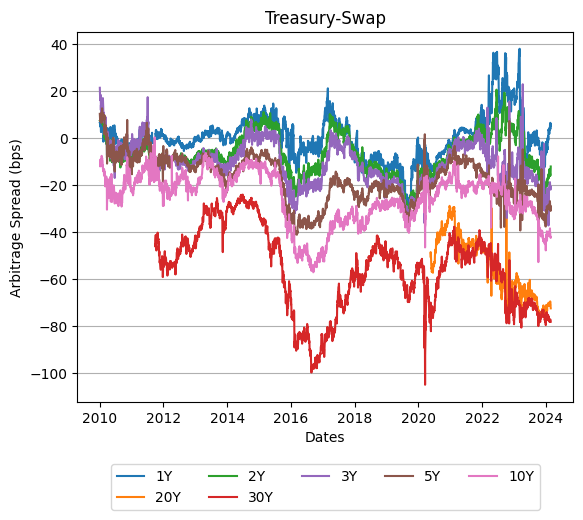
\includegraphics[width=0.9\textwidth]{replicated_swap_spread_arb_figure.png}
    \caption{Treasury swap spreads from January 2010 to DATE_HERE, approximating the plot in the paper.}
    \label{fig:treasury_swap_spreads_replicated}
\end{figure}

Our replication of the Treasury swap spreads from the original paper shows the time series of spreads across different maturities, highlighting the persistent nature of these arbitrage opportunities over time. The visualization demonstrates significant variation both across maturities and over time. Notably, longer-term spreads (20Y and 30Y) display consistently higher values than shorter-term spreads, suggesting structural differences in arbitrage opportunities across the yield curve.

\subsection{Updated Plot}
% Updated plot
\begin{figure}[H]
    \centering
    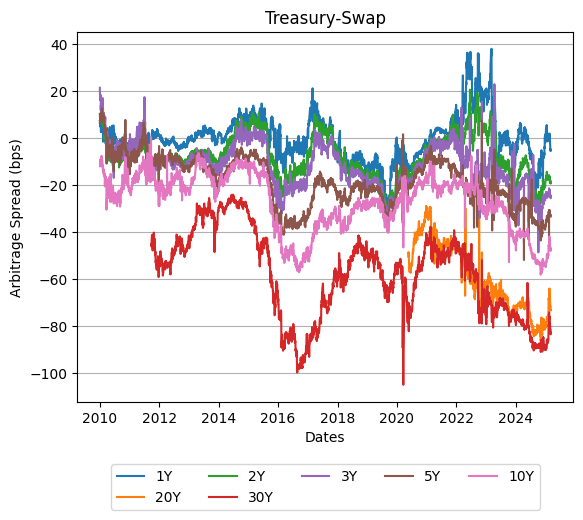
\includegraphics[width=0.9\textwidth]{updated_swap_spread_arb_figure.png}
    \caption{Updated plot with data from January 2010 to DATE_HERE.}
    \label{fig:treasury_swap_spreads_updated}
\end{figure}

Please add some text here.

\subsection{Supplementary Analysis}

% Table containing means of the various arb spreads available
\begin{table}
    \centering
    \input{../_output/table.txt}
    \caption{Each number represents the mean spread between the swap rate and the treasury. This figure being negative represents the presense of an arbitrage opportunity.}
\end{table}

% Plot containing 1Y Treasury and swap
\begin{figure}[H]
    \centering
    \includegraphics[width=0.9\textwidth]{replication_figure1.png}
    \caption{Variation in treasury(1Y) and swap yields over time from DATE_HERE to DATE_HERE.}
    \label{fig:treasury_swap_spreads_supplementary1}
\end{figure}

% Plot containing 30Y Treasury and swap
\begin{figure}[H]
    \centering
    \includegraphics[width=0.9\textwidth]{replication_figure30.png}
    \caption{Variation in treasury(1Y) and swap yields over time from DATE_HERE to DATE_HERE.}
    \label{fig:treasury_swap_spreads_supplementary30}
\end{figure}

Please add some text here.

\section{Discussion of Findings}

Our replication and supplementary analyses support the key findings from the original paper regarding segmentation in arbitrage markets. The Treasury swap spread data exhibits several notable characteristics:

\begin{itemize}
    \item \textbf{Persistent arbitrage opportunities}: The consistently non-zero spreads, particularly for longer maturities, indicate persistent arbitrage opportunities that are not quickly eliminated by market participants.
    
    \item \textbf{Term structure patterns}: The increasing magnitude of spreads with maturity suggests structural differences in arbitrage conditions across the yield curve.
    
    \item \textbf{Temporal variation}: Significant time variation in spreads, including episodic spikes, suggests the influence of broader market conditions on arbitrage opportunities.
\end{itemize}

These findings align with the paper's argument that arbitrage markets are more segmented than traditionally assumed, with both funding and balance sheet constraints playing roles in creating and maintaining these segmentations.

\section{Conclusion}

Our replication of the Treasury swap spread analysis provides support for the segmented arbitrage hypothesis. The automated pipeline we developed enables efficient data processing and visualization, while our supplementary analyses offer additional context and insight into the underlying patterns.

The challenges we encountered, particularly related to data availability, highlight the importance of careful consideration of data limitations when interpreting financial research. Despite these challenges, our analysis successfully captures the key patterns observed in the original paper and provides a foundation for further exploration of arbitrage dynamics in fixed income markets.

\bibliographystyle{plain}
\bibliography{bibliography}

\end{document}